\documentclass[]{article}
\usepackage{lmodern}
\usepackage{amssymb,amsmath}
\usepackage{ifxetex,ifluatex}
\usepackage{fixltx2e} % provides \textsubscript
\ifnum 0\ifxetex 1\fi\ifluatex 1\fi=0 % if pdftex
  \usepackage[T1]{fontenc}
  \usepackage[utf8]{inputenc}
\else % if luatex or xelatex
  \ifxetex
    \usepackage{mathspec}
  \else
    \usepackage{fontspec}
  \fi
  \defaultfontfeatures{Ligatures=TeX,Scale=MatchLowercase}
\fi
% use upquote if available, for straight quotes in verbatim environments
\IfFileExists{upquote.sty}{\usepackage{upquote}}{}
% use microtype if available
\IfFileExists{microtype.sty}{%
\usepackage{microtype}
\UseMicrotypeSet[protrusion]{basicmath} % disable protrusion for tt fonts
}{}
\usepackage[margin=1in]{geometry}
\usepackage{hyperref}
\hypersetup{unicode=true,
            pdftitle={Study on relationship between MPG and transmission type},
            pdfborder={0 0 0},
            breaklinks=true}
\urlstyle{same}  % don't use monospace font for urls
\usepackage{color}
\usepackage{fancyvrb}
\newcommand{\VerbBar}{|}
\newcommand{\VERB}{\Verb[commandchars=\\\{\}]}
\DefineVerbatimEnvironment{Highlighting}{Verbatim}{commandchars=\\\{\}}
% Add ',fontsize=\small' for more characters per line
\usepackage{framed}
\definecolor{shadecolor}{RGB}{248,248,248}
\newenvironment{Shaded}{\begin{snugshade}}{\end{snugshade}}
\newcommand{\KeywordTok}[1]{\textcolor[rgb]{0.13,0.29,0.53}{\textbf{#1}}}
\newcommand{\DataTypeTok}[1]{\textcolor[rgb]{0.13,0.29,0.53}{#1}}
\newcommand{\DecValTok}[1]{\textcolor[rgb]{0.00,0.00,0.81}{#1}}
\newcommand{\BaseNTok}[1]{\textcolor[rgb]{0.00,0.00,0.81}{#1}}
\newcommand{\FloatTok}[1]{\textcolor[rgb]{0.00,0.00,0.81}{#1}}
\newcommand{\ConstantTok}[1]{\textcolor[rgb]{0.00,0.00,0.00}{#1}}
\newcommand{\CharTok}[1]{\textcolor[rgb]{0.31,0.60,0.02}{#1}}
\newcommand{\SpecialCharTok}[1]{\textcolor[rgb]{0.00,0.00,0.00}{#1}}
\newcommand{\StringTok}[1]{\textcolor[rgb]{0.31,0.60,0.02}{#1}}
\newcommand{\VerbatimStringTok}[1]{\textcolor[rgb]{0.31,0.60,0.02}{#1}}
\newcommand{\SpecialStringTok}[1]{\textcolor[rgb]{0.31,0.60,0.02}{#1}}
\newcommand{\ImportTok}[1]{#1}
\newcommand{\CommentTok}[1]{\textcolor[rgb]{0.56,0.35,0.01}{\textit{#1}}}
\newcommand{\DocumentationTok}[1]{\textcolor[rgb]{0.56,0.35,0.01}{\textbf{\textit{#1}}}}
\newcommand{\AnnotationTok}[1]{\textcolor[rgb]{0.56,0.35,0.01}{\textbf{\textit{#1}}}}
\newcommand{\CommentVarTok}[1]{\textcolor[rgb]{0.56,0.35,0.01}{\textbf{\textit{#1}}}}
\newcommand{\OtherTok}[1]{\textcolor[rgb]{0.56,0.35,0.01}{#1}}
\newcommand{\FunctionTok}[1]{\textcolor[rgb]{0.00,0.00,0.00}{#1}}
\newcommand{\VariableTok}[1]{\textcolor[rgb]{0.00,0.00,0.00}{#1}}
\newcommand{\ControlFlowTok}[1]{\textcolor[rgb]{0.13,0.29,0.53}{\textbf{#1}}}
\newcommand{\OperatorTok}[1]{\textcolor[rgb]{0.81,0.36,0.00}{\textbf{#1}}}
\newcommand{\BuiltInTok}[1]{#1}
\newcommand{\ExtensionTok}[1]{#1}
\newcommand{\PreprocessorTok}[1]{\textcolor[rgb]{0.56,0.35,0.01}{\textit{#1}}}
\newcommand{\AttributeTok}[1]{\textcolor[rgb]{0.77,0.63,0.00}{#1}}
\newcommand{\RegionMarkerTok}[1]{#1}
\newcommand{\InformationTok}[1]{\textcolor[rgb]{0.56,0.35,0.01}{\textbf{\textit{#1}}}}
\newcommand{\WarningTok}[1]{\textcolor[rgb]{0.56,0.35,0.01}{\textbf{\textit{#1}}}}
\newcommand{\AlertTok}[1]{\textcolor[rgb]{0.94,0.16,0.16}{#1}}
\newcommand{\ErrorTok}[1]{\textcolor[rgb]{0.64,0.00,0.00}{\textbf{#1}}}
\newcommand{\NormalTok}[1]{#1}
\usepackage{graphicx,grffile}
\makeatletter
\def\maxwidth{\ifdim\Gin@nat@width>\linewidth\linewidth\else\Gin@nat@width\fi}
\def\maxheight{\ifdim\Gin@nat@height>\textheight\textheight\else\Gin@nat@height\fi}
\makeatother
% Scale images if necessary, so that they will not overflow the page
% margins by default, and it is still possible to overwrite the defaults
% using explicit options in \includegraphics[width, height, ...]{}
\setkeys{Gin}{width=\maxwidth,height=\maxheight,keepaspectratio}
\IfFileExists{parskip.sty}{%
\usepackage{parskip}
}{% else
\setlength{\parindent}{0pt}
\setlength{\parskip}{6pt plus 2pt minus 1pt}
}
\setlength{\emergencystretch}{3em}  % prevent overfull lines
\providecommand{\tightlist}{%
  \setlength{\itemsep}{0pt}\setlength{\parskip}{0pt}}
\setcounter{secnumdepth}{0}
% Redefines (sub)paragraphs to behave more like sections
\ifx\paragraph\undefined\else
\let\oldparagraph\paragraph
\renewcommand{\paragraph}[1]{\oldparagraph{#1}\mbox{}}
\fi
\ifx\subparagraph\undefined\else
\let\oldsubparagraph\subparagraph
\renewcommand{\subparagraph}[1]{\oldsubparagraph{#1}\mbox{}}
\fi

%%% Use protect on footnotes to avoid problems with footnotes in titles
\let\rmarkdownfootnote\footnote%
\def\footnote{\protect\rmarkdownfootnote}

%%% Change title format to be more compact
\usepackage{titling}

% Create subtitle command for use in maketitle
\newcommand{\subtitle}[1]{
  \posttitle{
    \begin{center}\large#1\end{center}
    }
}

\setlength{\droptitle}{-2em}
  \title{Study on relationship between MPG and transmission type}
  \pretitle{\vspace{\droptitle}\centering\huge}
  \posttitle{\par}
  \author{}
  \preauthor{}\postauthor{}
  \date{}
  \predate{}\postdate{}


\begin{document}
\maketitle

\section{Executive summary}\label{executive-summary}

In this report, the author investigated the relationship between MPG and
transmission type that appears in mtcars dataset by answering two
questions: 1. Is an automatic or manual transmission better for MPG, 2.
Quantify the MPG difference between automatic and manual transmission.
The linear regression model fitting was performed using transmission
type as the predictor for mpg. The model indicates that the manual cars
perform better in terms of mpg by 7.245 miles/gallon in average.
\#\#Exploratory data analysis\\
Following is an exploratory data analysis on the mtcar dataset.

\begin{Shaded}
\begin{Highlighting}[]
\CommentTok{# Load knitr library}
\KeywordTok{library}\NormalTok{(knitr)}
\KeywordTok{data}\NormalTok{(mtcars)}
\CommentTok{# Subset the data frame to have only "mpg" and "am" columns"}
\NormalTok{data <-}\StringTok{ }\NormalTok{mtcars[, }\KeywordTok{c}\NormalTok{(}\StringTok{"mpg"}\NormalTok{,}\StringTok{"am"}\NormalTok{)]}
\CommentTok{# Summary of the mtcars}
\KeywordTok{summary}\NormalTok{(data)}
\end{Highlighting}
\end{Shaded}

\begin{verbatim}
##       mpg              am        
##  Min.   :10.40   Min.   :0.0000  
##  1st Qu.:15.43   1st Qu.:0.0000  
##  Median :19.20   Median :0.0000  
##  Mean   :20.09   Mean   :0.4062  
##  3rd Qu.:22.80   3rd Qu.:1.0000  
##  Max.   :33.90   Max.   :1.0000
\end{verbatim}

\begin{Shaded}
\begin{Highlighting}[]
\CommentTok{# Observe the structure of the data}
\KeywordTok{str}\NormalTok{(data)}
\end{Highlighting}
\end{Shaded}

\begin{verbatim}
## 'data.frame':    32 obs. of  2 variables:
##  $ mpg: num  21 21 22.8 21.4 18.7 18.1 14.3 24.4 22.8 19.2 ...
##  $ am : num  1 1 1 0 0 0 0 0 0 0 ...
\end{verbatim}

We can observe various characteristics from the dataset. ``mpg''" column
has all the positive values with mean of 20.09. ``am'' is a binary
variable: 0 means automatic and 1 means manual transmission type. We
have 32 data points and each data point has information about mpg and
transmission type.\\
Furthermore, we can acquire a better understanding on the data by
plotting the data. ``mpg'' will be the dependant variable and ``am''"
will be the categorical independant variable. The boxplot (Plot A of
appendix) seems to suggest that manual transmission cars tend to have
higher mpg than the automatic cars.

\subsection{Linear regression model}\label{linear-regression-model}

\subsubsection{Model Fitting}\label{model-fitting}

Now we will fit linear regression model on mtcars dataset. Linear
regression model is chosen as the first model to use because it is the
most widely used and the result is easy to interpret. Furthermore the
outcome is conitunous data, so it makes most sense to use linear
regression model

\begin{Shaded}
\begin{Highlighting}[]
\CommentTok{# Linear model fit}
\NormalTok{lmfit <-}\StringTok{ }\KeywordTok{lm}\NormalTok{(mpg}\OperatorTok{~}\NormalTok{am, data)}
\KeywordTok{summary}\NormalTok{(lmfit)}\OperatorTok{$}\NormalTok{coefficients}
\end{Highlighting}
\end{Shaded}

\begin{verbatim}
##              Estimate Std. Error   t value     Pr(>|t|)
## (Intercept) 17.147368   1.124603 15.247492 1.133983e-15
## am           7.244939   1.764422  4.106127 2.850207e-04
\end{verbatim}

The linear regression result says that mpg = (17.127) + (7.245)*am. The
intercept is the expected mpg when the transmission type is automatic.
And the am coefficient means that mpg is expected to increase by 7.245
when the transmission is manual. The p-value for each coefficient is
very low. Therefore transmission type is a meaningful variable to
predict mpg. \#\#\#Diagnostic analysis and limitations However, the
R-squared value on the summary of the linear regression model is quite
low. It says that about 35\% of the mpg variability is explained by the
linear relationship with the am. Let's perform deeper diagnostic
analysis on the model

\begin{Shaded}
\begin{Highlighting}[]
\CommentTok{# lmfit coefficients confidence interval}
\KeywordTok{confint}\NormalTok{(lmfit)}
\end{Highlighting}
\end{Shaded}

\begin{verbatim}
##                2.5 %   97.5 %
## (Intercept) 14.85062 19.44411
## am           3.64151 10.84837
\end{verbatim}

The confidence interval for am coefficient is quite large. This is quite
concerning because 97.5\% value is three times the 2.5\% value. The
residual plot tells us that the residual values for manual transmission
data points are centered around below zero unlike that of automatic
transmission data points. Also the variance on the manual transmission
is larger than the other which makes us to suspect heteroscedasticity.
This tells us that this linear model is potentially underfitting and
should explore for other predictors.

\subsubsection{Conclusion - Answering the initial
questions}\label{conclusion---answering-the-initial-questions}

This study was initiated to answer the following questions: 1. Is an
automatic or manual transmission better for MPG, 2. Quantify the MPG
difference between automatic and manual transmission.\\
To answer both of these questions, we should look back to the and the
coefficient of the predictor. The sign of the coefficient is positive.
This means that manual cars tends to yield better mpg than the automatic
cars. Also the value 7.245 indicates that mpg is expected to increase by
that amount when the car is manual. Granted, the confidence interval of
the coefficient is quite big. However even at the lowest value in the
interval the value 3.642 indicates that mpg is expected to be better by
that amount for manual cars.

\subsection{Appendix}\label{appendix}

Plot A. Boxplot for explanatory data analysis

\begin{Shaded}
\begin{Highlighting}[]
\KeywordTok{library}\NormalTok{(ggplot2)}
\CommentTok{# Boxplot of the data}
\NormalTok{p <-}\StringTok{ }\KeywordTok{ggplot}\NormalTok{(data, }\KeywordTok{aes}\NormalTok{(}\DataTypeTok{x=}\KeywordTok{as.factor}\NormalTok{(am), }\DataTypeTok{y=}\NormalTok{mpg, }\DataTypeTok{color=}\KeywordTok{factor}\NormalTok{(am, }\DataTypeTok{labels =} \KeywordTok{c}\NormalTok{(}\StringTok{"0: Automatic"}\NormalTok{, }\StringTok{"1: Manual"}\NormalTok{)))) }\OperatorTok{+}\StringTok{ }\KeywordTok{geom_boxplot}\NormalTok{() }\OperatorTok{+}\StringTok{ }\KeywordTok{labs}\NormalTok{(}\DataTypeTok{title =} \StringTok{"Boxplot of mtcars data"}\NormalTok{)}\OperatorTok{+}\StringTok{ }\KeywordTok{xlab}\NormalTok{(}\StringTok{"Transmission"}\NormalTok{)}\OperatorTok{+}\KeywordTok{ylab}\NormalTok{(}\StringTok{"mpg"}\NormalTok{)}\OperatorTok{+}\KeywordTok{labs}\NormalTok{(}\DataTypeTok{color=}\StringTok{"Transmission Type"}\NormalTok{)}
\NormalTok{p}
\end{Highlighting}
\end{Shaded}

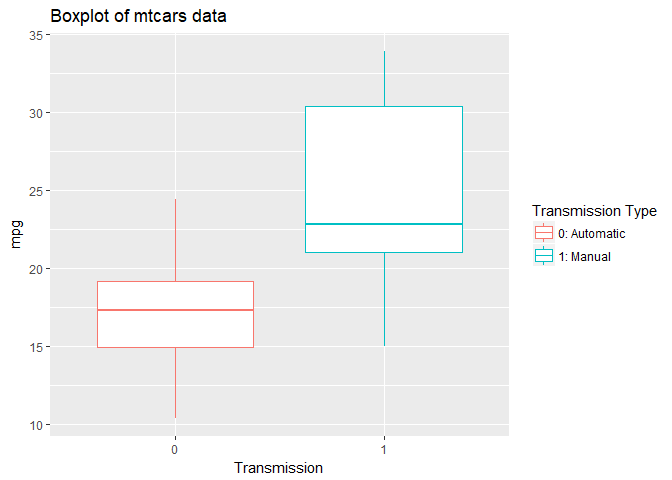
\includegraphics{final_project_files/figure-latex/unnamed-chunk-4-1.pdf}
Plot B. Residual plot for diagnostic analysis

\begin{Shaded}
\begin{Highlighting}[]
\CommentTok{# Residual plot of lmfit model}
\KeywordTok{plot}\NormalTok{(data}\OperatorTok{$}\NormalTok{am, }\KeywordTok{resid}\NormalTok{(lmfit), }\DataTypeTok{ylab=}\StringTok{"Residual plot"}\NormalTok{, }\DataTypeTok{xlab=}\StringTok{"mpg"}\NormalTok{, }\DataTypeTok{main =} \StringTok{"Residual vs am"}\NormalTok{)}
\end{Highlighting}
\end{Shaded}

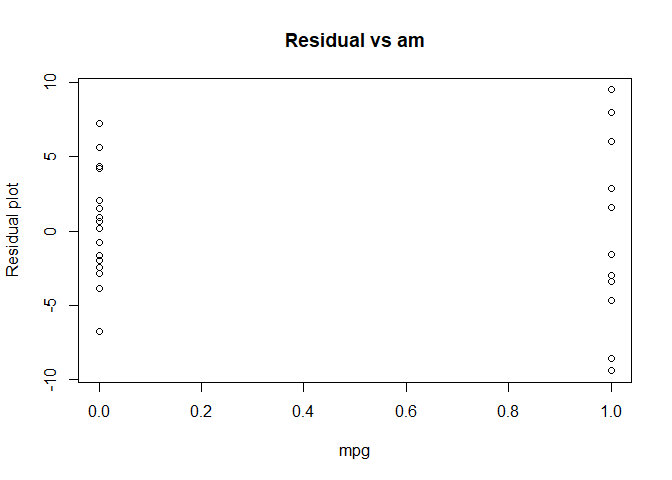
\includegraphics{final_project_files/figure-latex/unnamed-chunk-5-1.pdf}


\end{document}
